
\section{Context of the International Data Spaces}\label{sec:context}
%\addcontentsline{toc}{section}{Context of the International Data Spaces}
\subsection{Data-Driven Business Ecosystems and the Smart Service Welt}\label{subsec:data_driven_business_ecosystems}
%\addcontentsline{toc}{subsection}{Data-Driven Business Ecosystems and the Smart Service Welt}
Novel digital products and services often emerge in business ecosystems, which organizations enter to jointly fulfill the needs of customers better than they can do on their own. In such ecosystems, which emerge and dissolve much faster than traditional value creating networks, the partners have a clear focus on end-to-end customer processes in order to jointly develop innovative products and services. Actors in such ecosystems can be businesses (also direct competitors), research organizations, intermediaries (electronic marketplaces, for example), governmental agencies, and customers.

Ecosystems are characterized by the fact that no member is capable of creating innovation on its own. Instead, the ecosystem as a whole needs to team up. In other words: Every member has to contribute something for the benefit of all. Ideally, ecosystems function in an equilibrium state of mutual benefits for all members.

Examples of business ecosystems are numerous and can be found across all industries. Many of them have been analyzed and documented by the Smart Service Welt working group\footnote{ https://www.digitale-technologien.de/DT/Redaktion/DE/Downloads/Publikation/SSWII\_Programmbroschuere.pdf }.
%ToDo: update reference?

A data-driven business ecosystem is an ecosystem in which data is the strategic resource used by the members to jointly create innovative value offerings. Key to success is to share and jointly maintain data within such an ecosystem, as end-to-end customer process support can only be achieved if the partners team up and jointly utilize their data resource (as shown by a number of examples in Figure \ref{fig:_Data-Driven_Business_Ecosystems_examples}).


%%%%%%%%%%%%%%%%%%%% Figure/Image No: 5 starts here %%%%%%%%%%%%%%%%%%%%

\begin{figure}[H]
	\begin{Center}
		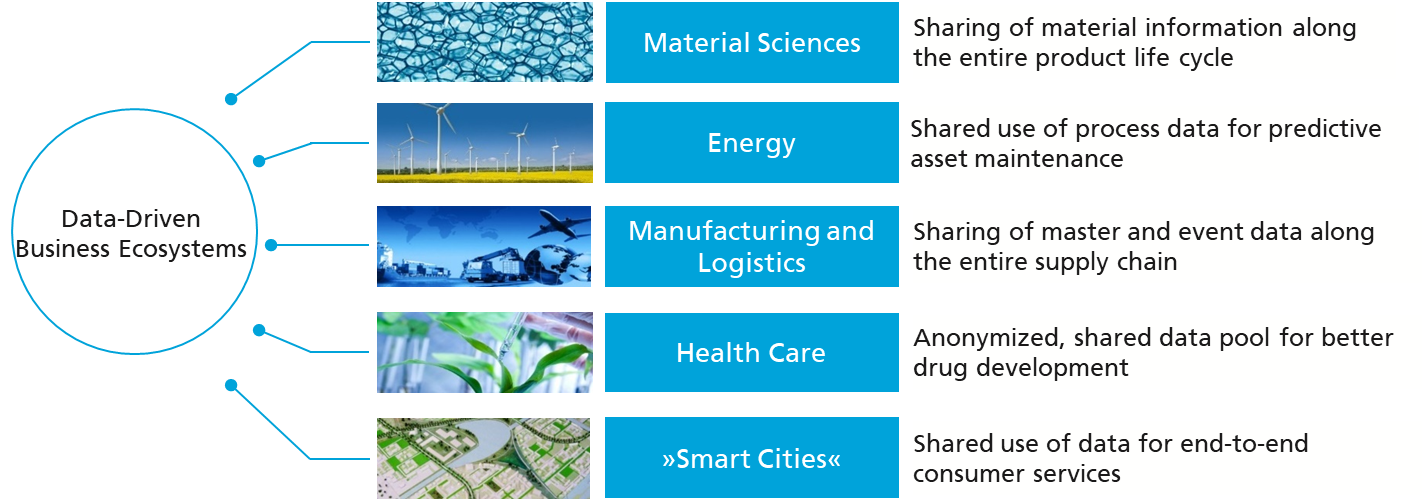
\includegraphics[width=6.42in,height=2.27in]{./media/image12.png}
		\caption{Data Sharing in Ecosystems}
		\label{fig:_Data-Driven_Business_Ecosystems_examples}
	\end{Center}
\end{figure}


%%%%%%%%%%%%%%%%%%%% Figure/Image No: 5 Ends here %%%%%%%%%%%%%%%%%%%%



\subsection{Data Sovereignty as a Key Capability}\label{subsec:datasovereignty_as_key_enabler}
%\addcontentsline{toc}{subsection}{Data Sovereignty as a Key Capability}
From these two developments – 1) data turning into a strategic resource, and 2) companies increasingly collaborating in business ecosystems – results a fundamental conflict of goals as a main characteristic of the digital economy: on the one hand, companies increasingly need to exchange data in business ecosystems; on the other hand, they feel they need to protect their data more than ever before, since the importance of data has grown so much. This conflict of goals is all the more intensified, the more a company is engaged in one or more business ecosystems, and the higher the value contributed by data to the overall success of the collaborative effort.

\textbf{Data sovereignty is about finding a balance between the need for protecting one’s data and the need for sharing one’s data with others. It can be considered a key capability for companies to develop in order to be successful in the data economy.}

To find that balance, it is important to take a close look at the data itself, as not all data requires the same level of protection, and as the value contribution of data varies, depending on what class or category it can be subsumed under.

\subsection{Data as an Economic Good}\label{subsec:data_as_economic_good}
%\addcontentsline{toc}{subsection}{Data as an Economic Good}
It is indisputable that data has a value, and that data management generates costs. Today, data is traded in the market like a commodity; it has a price, and many companies monitor the costs incurred for data management. However, data, being an intangible good, differs from tangible goods with regard to a number of properties, among which the fact that data is non-rival is considered the most important one. The value of data increases as it is being used (and, in many cases, as the number of user increases). While these differences hinder the adoption and application of legal provisions to the management and use of data, they do not dispute the fact that data is an economic good.

Depending on what type data is of, or what category it can be subsumed under, the value it contributes to the development of innovative products and services can vary. Therefore, the need for protection of data is not the same across all data types and data categories. Public data, for example, which can be accessed by anyone, requires a lower level of protection than private data or club data.

Because of these differences and distinctions made with regard to data, a generally accepted understanding of the value of data has not been established so far. Nevertheless, there is a growing need to determine the value of data, given the rapid developments taking place in the Smart Service Welt.

\subsection{Data Exchange and Data Sharing}\label{subsec:data_exchange_and_data_sharing}
%\addcontentsline{toc}{subsection}{Data Exchange and Data Sharing}
Cross-company data exchange with the help of inter-organizational information systems is not a new topic; it has been around for decades. With the proliferation of Electronic Data Interchange (EDI) in the 1980s, many different data exchange scenarios have emerged over time, which were accompanied by the development of certain technical standards.



%%%%%%%%%%%%%%%%%%%% Figure/Image No: 6 starts here %%%%%%%%%%%%%%%%%%%%

\begin{figure}[h]
	\begin{Center}
		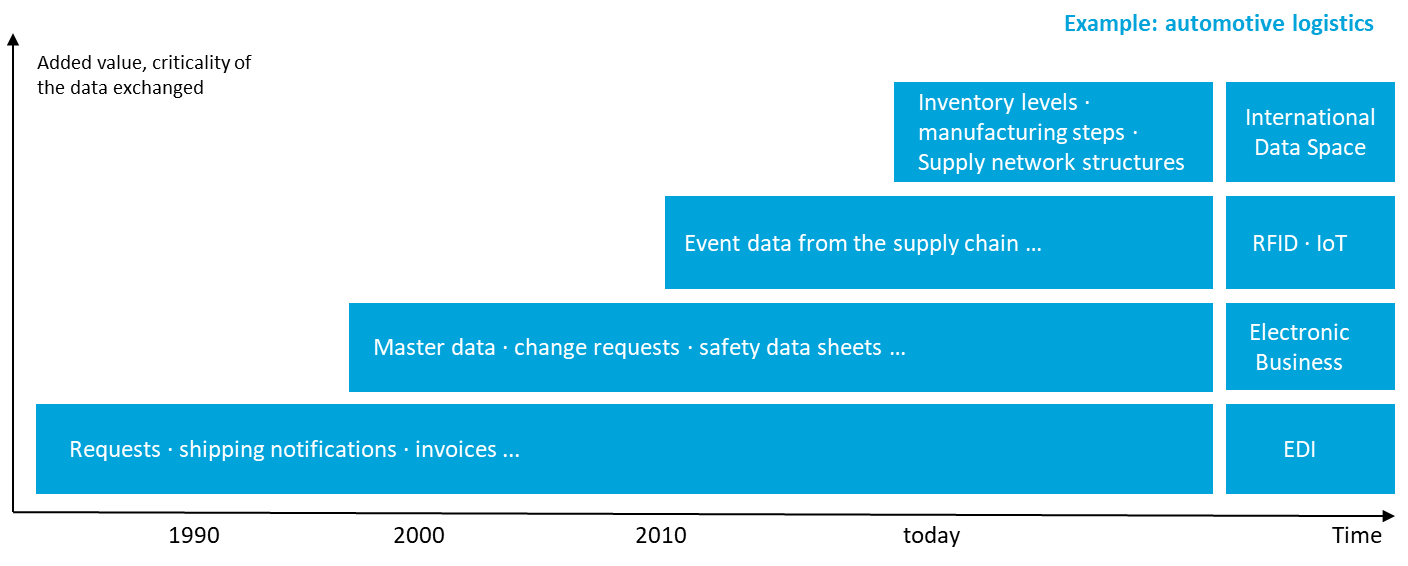
\includegraphics[width=6.67in,height=2.68in]{./media/image13.png}
		\caption{Evolution of technical standards for data exchange}
		\label{fig:Datadriven_business_ecosystems}
	\end{Center}
\end{figure}


%%%%%%%%%%%%%%%%%%%% Figure/Image No: 6 Ends here %%%%%%%%%%%%%%%%%%%%


Figure \ref{fig:Datadriven_business_ecosystems} shows the evolution of technical standards for data exchange since the 1980s, using the example of automotive logistics. Data sovereignty, which is one of the main goals of the International Data Spaces, materializes in $``$terms and conditions$"$  that are linked to data before it is exchanged and shared. However, these terms and conditions (such as time to live, forwarding rights, pricing information etc.) have not been standardized yet. In order to foster the establishment of data sovereignty in the exchange of data within business ecosystems, more standardization activities are needed.

This does not mean that existing standards will become obsolete. Instead, the overall set of standards companies need to comply with when exchanging and sharing data needs to be extended. It is therefore necessary to distinguish between data exchange and data sharing (see also Figure \ref{fig:dataexchange_vs_sharing}): 

\begin{itemize}
	\item Data exchange takes place in the \textit{vertical cooperation} between companies to support, enable or optimize value chains and supply chains (e.g. EDI messages in logistics or HL7 in medical scenarios).

	\item Data sharing takes place in the \textit{vertical and horizontal collaboration} between companies to achieve a common goal (e.g. predictive maintenance scenarios in manufacturing) or to enable new business models by generating additional value out of data (e.g. in data marketplaces). Furthermore, data sharing implies a mode of collaboration towards coopetition.

\end{itemize}



%%%%%%%%%%%%%%%%%%%% Figure/Image No: 7 starts here %%%%%%%%%%%%%%%%%%%%

\begin{figure}[H]
	\begin{Center}
		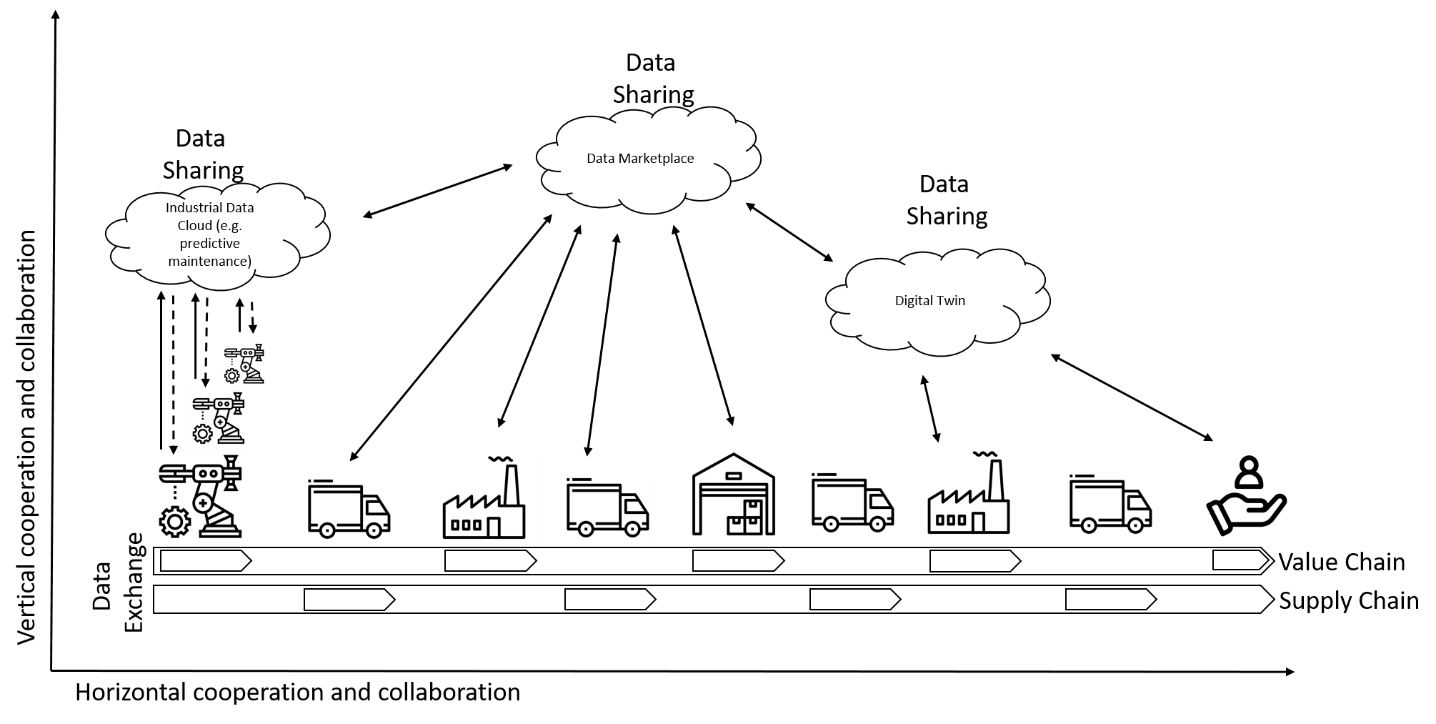
\includegraphics[width=6.53in,height=3.29in]{./media/image14.png}
		\caption{Data exchange vs. data sharing}
		\label{fig:dataexchange_vs_sharing}
	\end{Center}
\end{figure}


%%%%%%%%%%%%%%%%%%%% Figure/Image No: 7 Ends here %%%%%%%%%%%%%%%%%%%%

\subsection{Industrial Cloud Platforms}\label{subsec:industrial_cloud}
%\addcontentsline{toc}{subsection}{Industrial Cloud Platforms}
The growing number of industrial cloud platforms will also drive the need for a standard for data sovereignty. With a lot of different platforms emerging – driven by technology providers, software companies, system integrators, but also existing intermediaries – it is very likely that the platform landscape will be very heterogeneous, at least for some time. Platform providers will increasingly have to provide capabilities for secure and trusted data exchange and data sharing between their own platform and other platforms in the ecosystem.

Furthermore, the cloud platform landscape is likely to be characterized by a plurality of architectural patterns, ranging from approaches characterized by a high level of centralization (e.g. data lakes) to concepts promoting utmost decentralization (e.g. distributed applications using blockchain technology).

Which platform a data owner or data provider will choose to take advantage of will depend on the business criticality and the economic value of the data goods they want to exchange and share. As the data resource of a company consists of data of different criticality and value, it can be expected that many companies will use different platforms for different purposes.

%New: section on gaia x here
To make use of Cloud Platforms in industrial cases and maintain data sovereignty several prerequisites must be met. Especially in use cases, when different data providers bring together data in one cloud environment to be analyzed or used in general. The sovereign decision on a cloud environment must be enabled by interoperability in the perspective of data and in the perspective of the software, i.e. portability of a service into different cloud environments. In addition the capabilities of the service and the runtime must be transparent and verifiable to achieve trust in the cloud environment to be used. To achieve and to maintain interoperability and trust among the parties connected via a cloud environment a governance model must be provided and enforced in technology, in operative and administrative processes and  in legal agreements. 



\subsection{Big Data and Artificial Intelligence}\label{subsec:bigdata_ai}
%\addcontentsline{toc}{subsection}{Big Data and Artificial Intelligence}
Today companies make a wide use of Big Data applications. The common use case is to complement data available within the company by additional data (e.g. open data, data from other companies or data from data marketplaces). With the data portfolio extended this way, companies can benefit from significantly improved analytics results or from entirely new usage scenarios. 

Alongside with Big Data applications, also Artificial Intelligence (AI) applications have become more and more mature and powerful. Companies are increasingly using AI, which has led, and will continue to lead, to an even greater demand for external data (e.g. for training of AI models). However, companies often do not have sufficient data available in-house, which is why the need for data sharing with regard to using AI will rise.   

A standardized architecture for data exchange and data sharing would support the development and acceptance of both Big Data and AI applications in industry. At the same time, it is necessary to define usage policies for data sharing and retaining data sovereignty for data providers. 



\subsection{The Internet of Things and the Industrial Internet of Things}\label{subsec:iiot}
%\addcontentsline{toc}{subsection}{The Internet of Things and the Industrial Internet of Things}
The Internet of Things (IoT) and the Industrial Internet of Things (IIoT), respectively, comprises an ever-growing number of devices generating more and more data. While there is mostly a clear focus on the primary use of that data, it may be of interest for additional stakeholders as well. This requires standardization with regard to the (I)IoT architecture, but also standardization regarding data exchange and data sharing – in order to enable the data economy and facilitate the establishment of data marketplaces. The wide use of data generated within the (I)IoT will lead to new, smart and data centric services in conjunction with new business models.

\subsection{Blockchain}\label{subsec:blockchain}
%\addcontentsline{toc}{subsection}{Blockchain}
The core purpose of the International Data Spaces is to enable controlled exchange and sharing of data between organizations – regardless of the type of data. In many use cases of the International Data Spaces, this is some form of structured data (e.g. measurement data, product data, or logistics data). But also other types of (streaming) data are supported. The IDS Connector allows data owners and data providers to exchange and share their data with other participants in the IDS ecosystem, while data sovereignty is ensured at any time. 

In the use cases of the International Data Spaces, two basic patterns of data sharing can be found: 

\begin{itemize}
	\item Data is shared to feed new, data-driven services, such as using the data in a new app, smart algorithm, or other digital service in which data of different sources/providers is combined. 

	\item Data is shared for some form of business process synchronization, such as using the data to execute transactions (e.g. exchange orders), enable production (e.g. exchange product data), check quality (e.g. monitor the temperature of perishable goods), or synchronize processes (e.g. exchange status data). 
\end{itemize}

In many of these cases, this sharing of data enables transactions with the data itself becoming what one could call a ‘shared data asset’, resulting in liability/responsibility for the participating organizations. 

Two examples: 

\begin{itemize}
	\item As perishable goods were exposed to improper ambient temperatures, the company ordering the goods refuses acceptance. The temperature data thereby becomes a shared data asset that can be stored in a shared environment which acts as a trusted record keeper of such quality data. 

	\item Several companies want to share their capabilities in order to produce a certain type of good. In this case, the capability of each company becomes a shared data asset to be stored in shared ‘yellow pages’ accessible for all participants in the ecosystem. 
\end{itemize}

From a functional perspective, it is expected that blockchain technology will play an important role in maintaining these ‘shared data assets’ in an IDS environment. This would complement the existing capabilities of the IDS architecture to share (potentially large) datasets with the help of IDS Connectors. For instance, a shared data asset might encompass a hash code (‘fingerprint’ of a piece of data) which can be used to verify a larger file (e.g. a complex product design for which an order was sent) being shared with the help of an IDS Connector. In terms of the IDS-RAM, blockchain technology could be used for the Clearing House or the Broker, for example (see Business Layer).

In general, the use of Blockchain technology can ensure data consistency and transparency in combination with the general IDS approach for data sovereignty and secure data exchange and sharing. In contrast, typical Data Lakes focus on the integration of data for the purpose of knowledge extraction (see Figure \ref{fig:_general_architectural_patterns_for_data_exchange_and_data_sharing}).



%%%%%%%%%%%%%%%%%%%% Figure/Image No: 8 starts here %%%%%%%%%%%%%%%%%%%%

\begin{figure}[h]
	\begin{Center}
		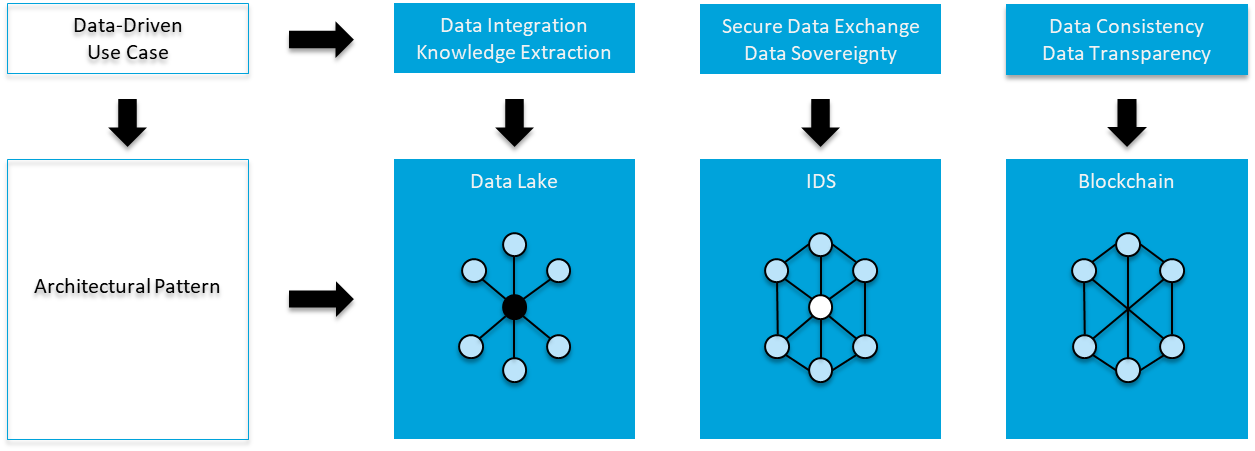
\includegraphics[width=6.6in,height=2.37in]{./media/image15.png}
		\caption{ General architectural patterns for data exchange and data sharing}
		\label{fig:_general_architectural_patterns_for_data_exchange_and_data_sharing}
	\end{Center}
\end{figure}


%%%%%%%%%%%%%%%%%%%% Figure/Image No: 8 Ends here %%%%%%%%%%%%%%%%%%%%

%new section for scheme owner

\subsection{Towards legal Interoperability: federated frameworks for data sharing agreements and terms-of-use}
\label{subsection:schemeowner}

IDS provides a federated data sharing environment. It poses strong requirements on interoperability on each of the levels as distinguished in the new European Interoperability Framework (as developed by the European Commission ): legal, organizational, semantic and technical interoperability under an overarching integrated governance approach.\\
Interoperability on the legal concepts applies to both the data sharing agreements (including legal, commercial and service level conditions) and the terms-of-use (i.e. the usage contracts consisting of access and usage policies). In practice, currently separate roles and organization are emerging providing services for the administration and registration of both data sharing agreements and terms-of-use, possibly under the same legal umbrella and specific for various data sharing communities. 
Within the current IDS role and interaction model, separate roles for managing data sharing agreements and terms-of-use are not distinguished (yet). Nevertheless, supporting such roles in a federated IDS environment is key to unambiguously understanding and agreement and adequately securing legal compliance for data sharing between organizations operating in different sectors, countries and jurisdictions.
In the co-operation between IDS and iSHARE\footnote{https://www.ishareworks.org/}, steps may be taken to address this challenge in defining the IDS approach to support federation of legal frameworks and semantic interoperability on legal conditions.


% end of new section


% new section on GDPR

\subsection{General Data Protection Regulation}
\label{subsec:gdpr}

Compliance of an organization to General Data Protection Regulation (GDPR) the  is only fulfilled by the implementation of both appropriate technical measures and appropriate organizational measures.

By participation of an organization in an IDS based ecosystem, the software which implements the IDS RAM can provide the technical measures. However, the responsibility and accountability with respect to GDPR compliance is on the part of the organization participating in the IDS ecosystem. This organization has to implement adequate organizational measures for the protection of personal data. This set of measures may be set up based on a risk assessment of personal data and personal data processing and - if the risk level exceeds certain thresholds - a data protection impact assessment.

Consequently, the organizations participating and their data processing within an IDS-based ecosystem have to be considered for GDPR compliance. Therefore, it cannot be said in general that IDS-RAM compliant leads to  GDPR-compliance. Instead, the role of IDS towards GDPR compliance should be in supporting the organizations participating in an IDS-based ecosystem through the implementation of technical measures and by giving advice about organizational measures. As a result, an IDS participant is enabled to set up GDPR-compliant processing and transfer of personal data within the scope of the IDS technology and features (see also: GDPR-related Requirements and Recommendations for the IDS Reference Architecture Model \footnote{TODO add link}).



% end of new section



\subsection{Contribution of the International Data Spaces to Industry 4.0 and the Data Economy}\label{subsec:contribution_to_industry40}
%\addcontentsline{toc}{subsection}{Contribution of the International Data Spaces to Industry 4.0 and the Data Economy}
By proposing an architecture for secure data exchange and trusted data sharing, the International Data Spaces contributes to the design of enterprise architectures in commercial and industrial digitization scenarios. It does so by bridging the gaps between research, industrial stakeholders, political stakeholders, and standards bodies. The architecture is designed with the objective to overcome the differences between top-down approaches and bottom-up approaches. Figure \ref{fig:5_Typical_enterprise_architecture_stack} shows a typical architecture stack of the digital industrial enterprise. The International Data Spaces connects the lower-level architectures for communication and basic data services with more abstract architectures for smart data services. It therefore supports the establishment of secure data supply chains from data source to data use, while at the same time making sure data sovereignty is guaranteed for data owners.



%%%%%%%%%%%%%%%%%%%% Figure/Image No: 9 starts here %%%%%%%%%%%%%%%%%%%%

\begin{figure}[h]
	\begin{Center}
		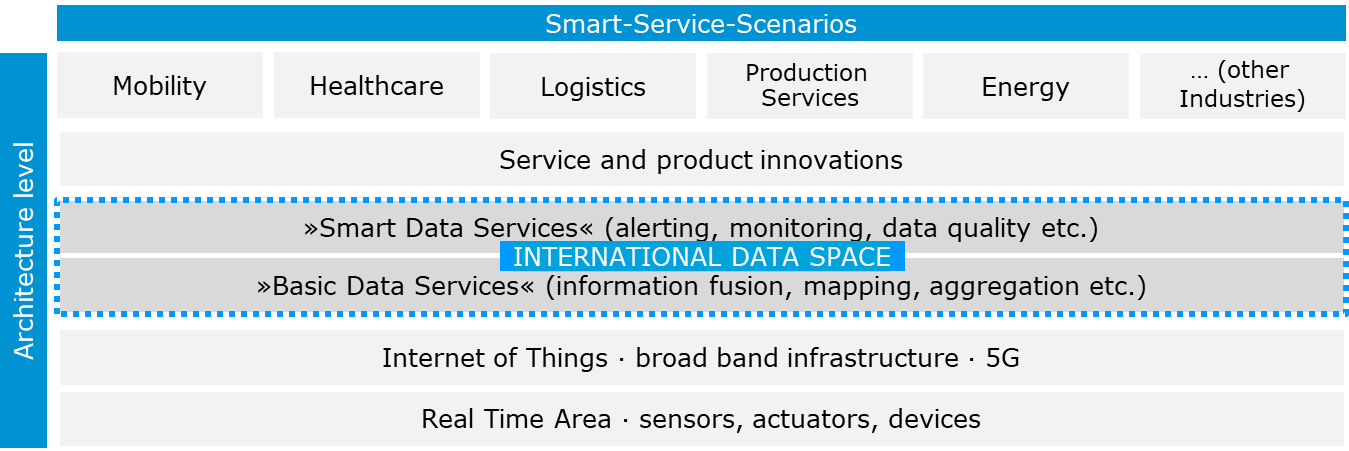
\includegraphics[width=6.25in,height=2.09in]{./media/image16.png}
		\caption{ Typical enterprise architecture stack}
		\label{fig:5_Typical_enterprise_architecture_stack}
	\end{Center}
\end{figure}


%%%%%%%%%%%%%%%%%%%% Figure/Image No: 9 Ends here %%%%%%%%%%%%%%%%%%%%



In broadening the perspective from an individual use case scenario to a platform landscape view, the International Data Spaces positions itself as an architecture that links different cloud platforms through policies and mechanisms for secure data exchange and trusted data sharing (or, in other words, through the principle of data sovereignty).\

Over the IDS Connector, the International Data Space’s central component, industrial data clouds, as well as individual enterprise clouds, on-premises applications and individual, connected devices can be connected to the International Data Spaces (see Figure \ref{fig:6_International_Data_Spaces_connecting_different_cloud_platforms}).



%%%%%%%%%%%%%%%%%%%% Figure/Image No: 10 starts here %%%%%%%%%%%%%%%%%%%%

\begin{figure}[h]
	\begin{Center}
		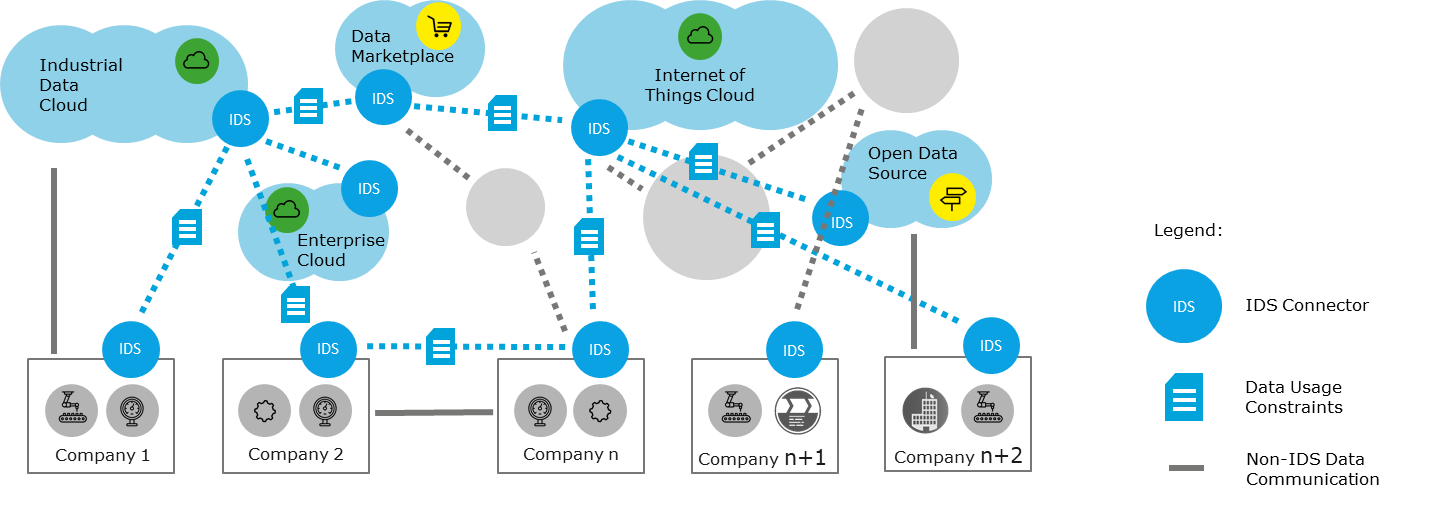
\includegraphics[width=6.42in,height=2.25in]{./media/image17.png}
		\caption{ International Data Spaces connecting different cloud platforms}
		\label{fig:6_International_Data_Spaces_connecting_different_cloud_platforms}
	\end{Center}
\end{figure}


%%%%%%%%%%%%%%%%%%%% Figure/Image No: 10 Ends here %%%%%%%%%%%%%%%%%%%%

With this integrating ambition, the International Data Spaces initiative positions itself in the context of cognate initiatives on both national and international level. Founded in Germany, the activities of the International Data Spaces are closely aligned with Plattform Industrie 4.0, in particular the Reference Architectures, Standards and Norms working group. 

The International Data Spaces initiative has established, and will continue to establish, liaisons with other initiatives, among them

%ToDo:update list
\begin{itemize}
	\item Alliance for Internet of Things Innovation,

	\item Big Data Value Association,

	\item Data Market Austria,

	\item Data Trading Alliance

	\item eCl@ss,

	\item FIWARE Foundation,

	\item Industrial Internet Consortium,

	\item iSHARE

	\item Industrial Valuechain Initative

	\item OPC Foundation,

	\item Plattform Industrie 4.0,

	\item Standardization Council Industrie 4.0, and

	\item World Wide Web Consortium.
\end{itemize}



Furthermore, the International Data Spaces initiative seeks collaboration and exchange of ideas with existing research and standardization initiatives. By functioning as a mediator between top-down and bottom-up approaches, bridging the gaps between research, industry, politics, and standards bodies, aligning the requirements of the economy and society, and fostering ties with other initiatives, the International Data Spaces can be considered a unique initiative in the landscape of \textit{Industry 4.0}.
